% Antecedentes del problema
%------------------------------------------------------------------

El comportamiento bursátil se caracteriza por mostrar movimientos oscilantes que dependen, no solo del valor real de las acciones, sino de la psicología de los inversores, tal como indican Ritter \cite{Ritter2003}, Sewell \cite{Sewell2010}, Shiller \cite{SHILLER1984} y Hu \cite{Hu2010}.\\

Este comportamiento volátil del mercado ha sido modelado y explicado por Weitert \cite{Christian2007} y Provenzano \cite{Provenzano2002}, como el resultado de la interacción entre los inversionistas guiados por el valor fundamental de las acciones y los inversores que siguen las tendencias, introduciendo las últimas alteraciones que desembocan en la volatilidad del mercado de valores.\\

% Problema
%------------------------------------------------------------------

Estar en capacidad de predecir el valor real de las empresas mineras permitiría a los inversores evitar perder su dinero debido a la volatilidad del mercado.\\

% Justificacion
%------------------------------------------------------------------

El mercado bursátil, en el Perú y en el mundo, cumple una importante función como herramienta de inversión y jubilación, para inversionistas individuales, fondos mutuos y fondos de pensiones. Por ejemplo, en el Perú, el 2011 había cerca de cinco millones de afiliados al Sistema Privado de Pensiones (SPP) -tal como se puede observar en la figura \ref{graf:afiliados-spp} \cite{AFP2011} - quienes dependen, en un porcentaje variable según el fondo, del mercado de valores para sus fines previsionales.\\


\begin{figure*}
   \centering
   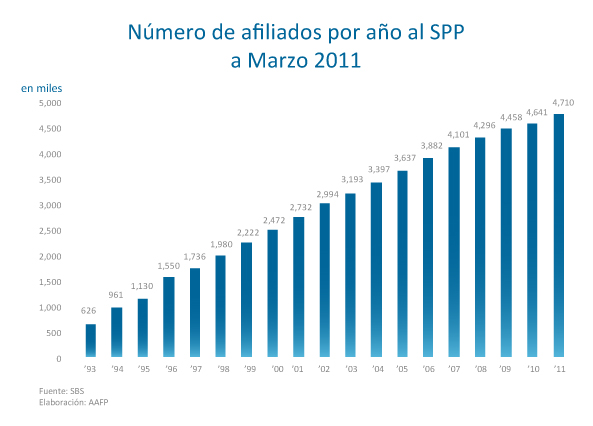
\includegraphics[scale=0.7]{imagenes/afiliados-marzo-2011.jpg}
   \caption{Afiliados al SPP \cite{AFP2011}}\label{graf:afiliados-spp}
\end{figure*}



% Estado del arte
%------------------------------------------------------------------

Diversos autores han tratado el problema de predecir la tendencia de los precios en el mercado bursátil, basandose en el análisis de los estados financieros. Benjamin Graham \cite{BenjaminGraham2009}, \cite{Graham2007} y David Dodd son considerados los fundadores del análisis de los fundamentos o análisis fundamental.\\

Basados en el análisis fundamental, investigadores como	Lev \& Thiagarajan, Abarbanell \& Bushee y Piotroski han creado modelos para predecir el cambio en la utilidades de una empresa basándose en indicadores financieros y contables.\\

% Organización
%------------------------------------------------------------------

Lo que resta del artículo se organiza como sigue: se llevará a cabo una exposición resumida de las propuestas más recientes en cuanto a modelos de predicción basados en el análisis fundamental y una exposición detallada de cada modelo, para terminar se llevará a cabo una comparación entre los diversos modelos y se expondrán las conclusiones.\\
